\documentclass[12pt]{article}
\usepackage{amsmath}
\usepackage{amssymb}
\usepackage[letterpaper,top=0.75in,bottom=1in,left=0.75in,right=0.75in,centering]{geometry}
%\usepackage{fancyhdr}
\usepackage{enumerate}
%\usepackage{lastpage}
\usepackage{multicol}
\usepackage{graphicx}
\usepackage{tikz}
\usetikzlibrary{calc, positioning, decorations.pathmorphing}

\reversemarginpar

%\pagestyle{fancy}
%\cfoot{}
%\lhead{Math 1560}\chead{Test \# 1}\rhead{May 18th, 2017}
%\rfoot{Total: 10 points}
%\chead{{\bf Name:}}
\newcommand{\points}[1]{\marginpar{\hspace{24pt}[#1]}}
\newcommand{\skipline}{\vspace{12pt}}
%\renewcommand{\headrulewidth}{0in}
\headheight 30pt

\newcommand{\di}{\displaystyle}
\newcommand{\abs}[1]{\lvert #1\rvert}
\newcommand{\len}[1]{\lVert #1\rVert}
\renewcommand{\i}{\mathbf{i}}
\renewcommand{\j}{\mathbf{j}}
\renewcommand{\k}{\mathbf{k}}
\newcommand{\R}{\mathbb{R}}
\newcommand{\aaa}{\mathbf{a}}
\newcommand{\bbb}{\mathbf{b}}
\newcommand{\ccc}{\mathbf{c}}
\newcommand{\dotp}{\boldsymbol{\cdot}}
\newcommand{\bbm}{\begin{bmatrix}}
\newcommand{\ebm}{\end{bmatrix}}                   
                  
\begin{document}


\author{Instructor: Sean Fitzpatrick}
\thispagestyle{empty}
\vglue1cm
\begin{center}
{\bf MATH 1560 - Tutorial \#6 Solutions}
\end{center}

\textbf{Assigned problems:}
\begin{enumerate}
\item Determine the global maximum and minimum values of the given function on the given interval. (Note: these values can occur at either a critical number or an end point.)
\begin{enumerate}
\item $f(x)=x^3-x^2$, on $[-1,2]$.

First, we compute $f(-1)=-1-1=-2$ and $f(2)=8-4=4$. Next, we find
\[
f'(x) = 3x^2-2x=x(3x-2),
\]
so $f'(x)=0$ for $x=0$ and $x=2/3$. We have $f(0)=0$, and $f(2/3) = \dfrac{8}{27}-\dfrac{4}{9} = -\dfrac{4}{27}$.

Notice that $-2<-4/27<0<4$, so the absolute minimum is $f(-1)=-2$, and the absolute maximum is $f(2)=4$.

\item $g(x) = 3x^{2/3}-2x$, on $[-1,8]$.

We begin with the endpoints. $g(-1) = 3(1)-2(-1)=5$, and $g(8)=3(4)-2(8)=-4$. Now we check the critical points:
\[
g'(x) = 2x^{-1/3}-2=2x^{-1/3}(1-x^{1/3}).
\]
Thus, $g'(x)=0$ if $x=1$, and $g'(x)$ is undefined when $x=0$. Since 0 is in the domain of $g$, both of these are critical points. We find $g(1)=3-2=1$ and $g(0)=0-0=0$.

Since $-4<0<1<5$, the absolute minimum is at $(8,-4)$, and the absolute maximum is at $(-1,5)$.


\end{enumerate}

\item  Determine the intervals on which $f(x) = \dfrac{x^2+3}{x-1}$ is increasing and decreasing.

The derivative of $f$ is given by
\[
f'(x) = \frac{2x(x-1)-(x^2+3)(1)}{(x-1)^2} = \frac{x^2-2x-3}{(x-1)^2}=\frac{(x+1)(x-3)}{(x-1)^2}.
\]
Thus, $f'(x) = 0$ when $x=-1$ and $x=3$, and $f'(x)$ is undefined at the  vertical asymptote $x=1$. We plot these points on a number line and determine the sign between each one:

    \begin{center}
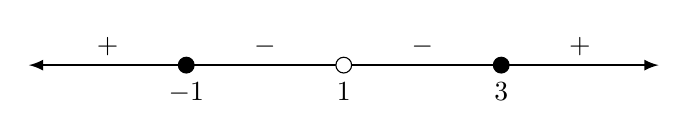
\begin{tikzpicture}[>=latex]
  \draw [thick, <->] (-4,0) -- (4,0);
  \draw [fill] (-2,0) circle [radius =.1];
  \draw [fill=white] (0,0) circle [radius =.1];
  \draw [fill] (2,0) circle [radius =.1];
  \node at (-3,0) [above] {$+$};
  \node at (-1,0) [above] {$-$};
  \node at (1,0) [above] {$-$};
  \node at (3,0) [above] {$+$};
  \node at (-2,-0.1) [below] {$-1$};
  \node at (0,-0.1) [below] {$1$};
  \node at (2,-0.1) [below] {$3$};
  \end{tikzpicture}
\end{center}

From the sign diagram, we see that $f'(x)>0$, and thus $f$ is increasing, on $(-\infty,-1)\cup (3,\infty)$, while $f'(x)<0$, and thus $f$ is decreasing, on $(-1,1)\cup (1,3)$.

\textbf{Note:} Since $f(1)$ is undefined, we should not include $x=1$ in any of our intervals. Thus, we write $(-1,1)\cup (1,3)$ for the intervals of decrease, rather than $(-1,3)$.

\newpage

\item Sketch the graph of $f(x) = (x-3)\sqrt{x}$. 

\begin{itemize}
\item Due to the square root, the domain of $f$ is $[0,\infty)$. The $x$-intercepts are $(0,0)$ (also the $y$-intercept) and $(3,0)$.

\item There are no asymptotes. We have $f(0)=0$ from the above, and as $x\to \infty$, $f(x)\to\infty$.

\item Writing $f(x) = x^{3/2}-3x^{1/2}$, we have
\[
f'(x) = \frac32 x^{1/2}-\frac32 x^{-1/2} = \frac{3(x-1)}{2\sqrt{x}}.
\]
We see that $f'(1)=0$, and $f'(0)$ is undefined. The sign diagram looks like:
\begin{center}
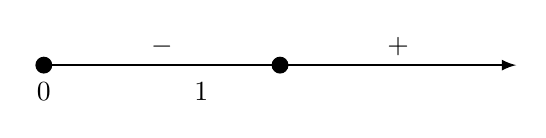
\begin{tikzpicture}[>=latex]
  \draw [thick, ->] (-2,0) -- (4,0);
  \draw [fill] (-2,0) circle [radius =.1];
  \draw [fill] (1,0) circle [radius =.1];
  \node at (-0.5,0) [above] {$-$};
  \node at (2.5,0) [above] {$+$};
  \node at (-2,-0.1) [below] {$0$};
  \node at (0,-0.1) [below] {$1$};
  \end{tikzpicture}
\end{center}
Thus $f$ is decreasing on $(0,1)$, increasing on $(1,\infty)$, and there is a local minimum at $(1,f(1))=(1,-2)$.

Note also that $\di \lim_{x\to 0^+}f'(x) = -\infty$, which tells us that the slope of the tangent line is large and negative when $x$ is near zero, and the tangent line approaches vertical at the origin.

\item Note that it is much easier to compute $f''(x)$ using the unfactored expression for $f'(x)$ above (power rule is easier than quotient rule). We have
\[
f''(x) = \frac34 x^{-1/2}+\frac34 x^{-3/2},
\]
and we note that $f''(x)>0$ for all $x>0$, and thus there are no inflection points, and the entire graph of $f$ is concave up.

To plot the graph, we mark the intercepts $(0,0)$ and $(3,0)$, the turning point $(1,-2)$, and we connect the dots, making sure that the tangent looks close to vertical near the origin, and that the graph is concave up throughout. The result should look like the following:
\begin{center}
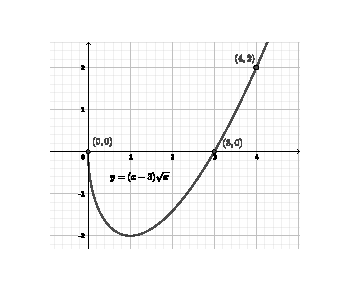
\includegraphics[width=0.6\textwidth]{Tut6-3sol}
\end{center}
\end{itemize}

\newpage


\item Extra fun: The graph of the \textit{derivative} of a \textbf{continuous} function $f$ is given below. From the graph, determine:
\begin{multicols}{2}
\begin{enumerate}
\item The intervals on which $f$ is increasing/decreasing.
\item The $x$-coordinates of any local maxima or minima.
\item The intervals on which $f$ is concave up/down.
\item The $x$-coordinates of any inflection points.
\item A rough graph of $f$, assuming that $f(0)=0$.
\end{enumerate}
\begin{center}
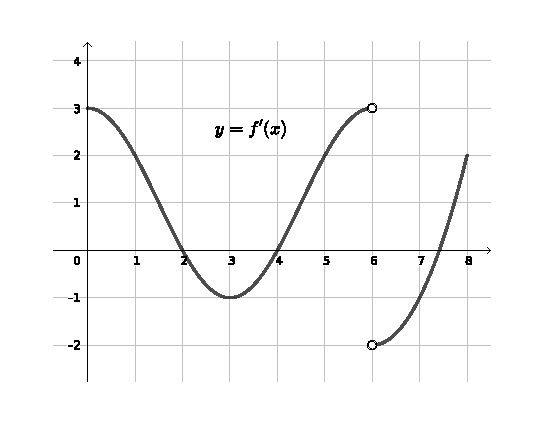
\includegraphics[width=\columnwidth]{Tut6-4}
\end{center}
\end{multicols}

From the graph of $f'(x)$ we can determine its sign diagram, by noting where $f'(x)>0$ (the graph is above the $x$-axis), and where $f'(x)<0$ (the graph is below the $x$-axis). We find (approximating the root of $f'(x)$ between 7 and 8 to be at $7.3$:
\begin{center}
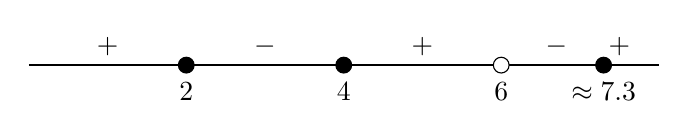
\begin{tikzpicture}[>=latex]
  \draw [thick, -] (0,0) -- (8,0);
  \draw [fill] (2,0) circle [radius =.1];
  \draw [fill=white] (6,0) circle [radius =.1];
  \draw [fill] (4,0) circle [radius =.1];
  \draw [fill] (7.3,0) circle [radius =.1];
  \node at (1,0) [above] {$+$};
  \node at (5,0) [above] {$+$};
  \node at (6.7,0) [above] {$-$};
  \node at (3,0) [above] {$-$};
  \node at (7.5,0) [above] {$+$};
  \node at (2,-0.1) [below] {$2$};
  \node at (4,-0.1) [below] {$4$};
  \node at (6,-0.1) [below] {$6$};
  \node at (7.3,-0.1) [below] {$\approx 7.3$};
  \end{tikzpicture}
\end{center}
From this we see that $f$ is increasing on $[0,2]\cup [4,6]\cup [7.3,8]$ and decreasing on $[2,4]\cup [6,7.3]$. 

The critical numbers are $x=2$ (local max), $x=4$ (local min), $x=6$, ($f'(6)$ does not exist, but we're told that $f$ is continuous, so this must be a critical number, and in this case, it's a local max), and $x=7.3$ (local min). 

We know that the graph of $f$ will be concave up where $f''(x)>0$, and concave down where $f''(x)<0$. Since $f''(x)$ is the derivative of $f'(x)$, we can conclude that $f''(x)>0$ where $f'(x)$ is increasing, and $f''(x)<0$ where $f'(x)$ is decreasing. 

Our sign diagram is as follows:
\begin{center}
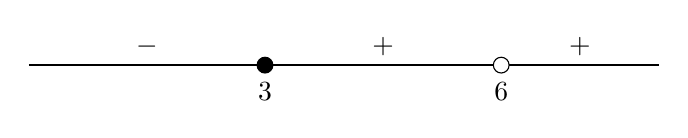
\begin{tikzpicture}[>=latex]
  \draw [thick, -] (0,0) -- (8,0);
  \draw [fill] (3,0) circle [radius =.1];
  \draw [fill=white] (6,0) circle [radius =.1];
  \node at (1.5,0) [above] {$-$};
  \node at (4.5,0) [above] {$+$};
  \node at (7,0) [above] {$+$};
  \node at (3,-0.1) [below] {$3$};
  \node at (6,-0.1) [below] {$6$};
  \end{tikzpicture}
\end{center}
We see that the graph of $f$ is concave up on $[3,6)\cup (6,8]$, and concave down on $[0,3]$. 

There is one point of inflection, when $x=3$.

To plot the graph, we have to guess at the $y$-coordinates of the turning points and inflection points, since it's impossible to find these without knowing the function $f$. (For example, we could add any constant to $f$ without changing the derivative.) One possible graph is as follows:
\begin{center}
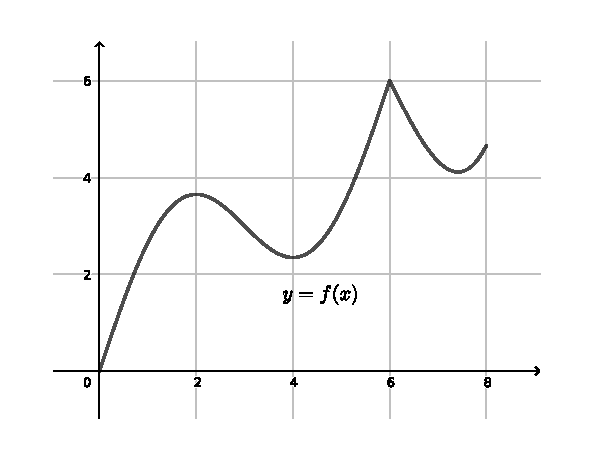
\includegraphics[width=0.6\textwidth]{Tut6-4sol}
\end{center}
  \end{enumerate}
  \newpage
  
\textbf{Additional practice problems:}
\begin{enumerate}
\item Find the absolute (global) maximum and minimum values of the given function on the given interval:
\begin{enumerate}
\item $f(x) = x^2\sqrt{4-x^2}$, on $[-2,2]$.

Note that $f(2)=f(-2)=0$. We have
\[
f'(x) = 2x\sqrt{4-x^2}+x^2\left(\frac{-2x}{2\sqrt{4-x^2}}\right)=\frac{2x(4-x^2)-x^3}{\sqrt{4-x^2}}=\frac{x(8-3x^2)}{\sqrt{4-x^2}}.
\]
We find that $f'(x)$ is undefined at the endpoints, $x=\pm 2$, but we've already checked these values. In addition, $f'(x)=0$ for $x=0$ and $x=\pm\sqrt{8/3}$. The corresponding $y$ values are $f(0)=0$ and
\[
f(\sqrt{8/3}) = \frac{8}{3}\sqrt{4-8/3} = \frac{8}{3}\sqrt{4/3}=\frac{16}{3\sqrt{3}}=f(-\sqrt{8/3}).
\]
Thus, the absolute minimum is $0$, which is obtained at $x=-2,0,2$, and the absolute maximum is $\dfrac{16}{3\sqrt{3}}$, which is obtained at $x=\pm \sqrt{8/3}$.

(You may wish to verify this by having a computer plot the graph of the function.)

\item $g(x) = x+\dfrac{3}{x}$, on $[1,5]$.

At the end points, we have $g(1) = 1+3=4$ and $g(5) = 5+\frac{3}{5}=\frac{28}{5}$.

The derivative is
\[
g'(x) = 1-\frac{3}{x^2} = \frac{x^2-3}{x^2} = \frac{(x-\sqrt{3})(x+\sqrt{3})}{x^2}.
\]
We see that $g'(x)=0$ for $x=\pm \sqrt{3}$, but only $x=\sqrt{3}$ is in the interval $[1,5]$. We find
\[
g(\sqrt{3}) = \sqrt{3}+\frac{3}{\sqrt{3}}=\sqrt{3}+\sqrt{3}=2\sqrt{3}.
\]
We now need to compare the values $4$, $\dfrac{28}{5}$, and $2\sqrt{3}$. Clearly $4=\frac{20}{5}<\frac{28}{5}$, and since $(2\sqrt{3})^2 = 4\cdot 3=12<16=4^2$, we see that the absolute minimum is $2\sqrt{3}=f(\sqrt{3})$, and the absolute maximum is $\dfrac{28}{5}=f(5)$.

\item $h(x) = e^x\sin(x)$, on $[0,\pi]$

At the end points, we have $h(0)=h(\pi)=0$. The derivative is
\[
h'(x) = e^x\sin(x)+e^x\cos(x)=e^x(\sin(x)+\cos(x)).
\]
Since $e^x\neq 0$ for all $x$, $h'(x)=0$ when $\sin(x)+\cos(x)=0$, which is equivalent to $\sin(x)=-\cos(x)$ or $\tan(x)=-1$. The only value of $x$ in $[0,\pi]$ that solves this equation is $x=3\pi/4$. We find
\[
h(3\pi/4) = e^{3\pi/4}\sin(3\pi/4) = \frac{e^{3\pi/4}}{\sqrt{2}}.
\]
Since this value is positive, it must be the absolute maximum, and the absolute minimum is zero, which is attained at either end point.
\end{enumerate}

\item Find all critical numbers for each function, and determine if each one is a local maximum, local minimum, or neither:
\begin{enumerate}
\item $f(x)=x^4-6x^2+4$

The derivative is
\[
f'(x) = 4x^3-12x=4x(x^2-3)=4x(x-\sqrt{3})(x+\sqrt{3}).
\]
The critical numbers are thus $x=0$, $x=\sqrt{3}$, and $x=-\sqrt{3}$. A sign diagram is given by
\begin{center}
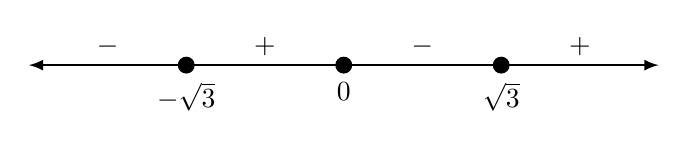
\begin{tikzpicture}[>=latex]
  \draw [thick, <->] (-4,0) -- (4,0);
  \draw [fill] (-2,0) circle [radius =.1];
  \draw [fill] (0,0) circle [radius =.1];
  \draw [fill] (2,0) circle [radius =.1];
  \node at (-3,0) [above] {$-$};
  \node at (-1,0) [above] {$+$};
  \node at (1,0) [above] {$-$};
  \node at (3,0) [above] {$+$};
  \node at (-2,-0.1) [below] {$-\sqrt{3}$};
  \node at (0,-0.1) [below] {$0$};
  \node at (2,-0.1) [below] {$\sqrt{3}$};
  \end{tikzpicture}
\end{center}
From the sign diagram, we see that $f$ has local minima at $\pm \sqrt{3}$ (the derivative changes from negative to positive, so $f$ changes from decreasing to increasing), and a local maximum at 0 (the derivative changes from positive to negative, so $f$ changes from increasing to decreasing.)

The $y$ values are given by $f(\pm\sqrt{3}) = 9-18+4=-5$ and $f(0)=4$.

\item $g(x) = x^3\ln(x)$

We compute
\[
g'(x) = 3x^2\ln(x)+x^3(1/x) = 3x^2\ln(x)+x^2=x^2(3\ln(x)+1).
\]
Since 0 is not in the domain of $g$ (recall that $\ln(x)$ is only defined for $x>0$), our only critical point is obtained when $3\ln(x)+1=0$. This is equivalent to $\ln(x)=-1/3$, or $x=e^{-1/3}$.

Note the graph of $3\ln(x)+1$ looks the same as the graph of $\ln(x)$, but stretched vertically by a factor of 3, and shifted up one unit. This tells us that $3\ln(x)+1$ is increasing everywhere, so it must be negative when $x<e^{-1/3}$  and positive when $x>e^{-1/3}$.

It follows that the graph of $g$ switches from decreasing to increasing at $e^{-1/3}$, so there is a local minimum at this point.

The $y$-value is $g(e^{-1/3}) = (e^{-1/3})^2\ln(e^{-1/3})=-\frac{1}{3e^{2/3}}.$

\item $h(x) = x^2e^{-2x}$

We start with the derivative:
\[
h'(x) = 2xe^{-2x}+x^2(-2e^{-2x})=e^{-2x}(2x-2x^2)=2xe^{-2x}(1-x),
\]
so $h'(x)=0$ for $x=0$ and $x=1$. Since $e^{-2x}>0$ everywhere, our sign diagram is given by
\begin{center}
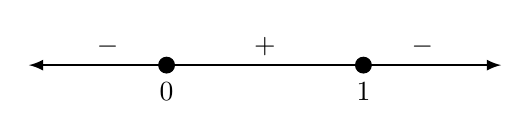
\begin{tikzpicture}[>=latex]
  \draw [thick, <->] (-3,0) -- (3,0);
  \draw [fill] (-1.25,0) circle [radius =.1];
  \draw [fill] (1.25,0) circle [radius =.1];
  \node at (-2,0) [above] {$-$};
  \node at (0,0) [above] {$+$};
  \node at (2,0) [above] {$-$};
  \node at (-1.25,-0.1) [below] {$0$};
  \node at (1.25,-0.1) [below] {$1$};
  \end{tikzpicture}
\end{center}
From the sign diagram, we see that $(0,h(0))=(0,0)$ is a local minimum, and $(1,h(1))=(1,e^{-2})$ is a local maximum.
\end{enumerate}
\end{enumerate}








\end{document}